% This must be in the first 5 lines to tell arXiv to use pdfLaTeX, which is strongly recommended.
\pdfoutput=1
% In particular, the hyperref package requires pdfLaTeX in order to break URLs across lines.

\documentclass{article}

% if you need to pass options to natbib, use, e.g.:
%     \PassOptionsToPackage{numbers, compress}{natbib}
% before loading neurips_2026

% The authors should use one of these tracks.
% Before accepting by the NeurIPS conference, select one of the options below.
% 0. "default" for submission
% \usepackage{neurips_2026}
% the "default" option is equal to the "main" option, which is used for the Main Track with double-blind reviewing.
% 1. "main" option is used for the Main Track
% \usepackage[main]{neurips_2026}
% 2. "position" option is used for the Position Paper Track
%  \usepackage[position]{neurips_2026}
% 3. "eandd" option is used for the Evaluations & Datasets Track
% \usepackage[eandd]{neurips_2026}
% if you want to opt-in for a de-anomymized submission (not recommended, but OK):
%\usepackage[eandd, nonanonymous]{neurips_2026}
% 4. "creativeai" option is used for the Creative AI Track
%  \usepackage[creativeai]{neurips_2026}
% 5. "sglblindworkshop" option is used for the Workshop with single-blind reviewing
% \usepackage[sglblindworkshop]{neurips_2026}
% 6. "dblblindworkshop" option is used for the Workshop with double-blind reviewing
%  \usepackage[dblblindworkshop]{neurips_2026}

% After being accepted, the authors should add "final" behind the track to compile a camera-ready version.
% 1. Main Track
\usepackage[main, final]{neurips_2026}
% 2. Position Paper Track
%  \usepackage[position, final]{neurips_2026}
% 3. Evaluations & Datasets Track
% \usepackage[eandd, final]{neurips_2026}
% 4. Creative AI Track
%  \usepackage[creativeai, final]{neurips_2026}
% 5. Workshop with single-blind reviewing
%  \usepackage[sglblindworkshop, final]{neurips_2026}
% 6. Workshop with double-blind reviewing
%  \usepackage[dblblindworkshop, final]{neurips_2026}
% Note. For the workshop paper template, both \title{} and \workshoptitle{} are required, with the former indicating the paper title shown in the title and the latter indicating the workshop title displayed in the footnote.
% For workshops (5., 6.), the authors should add the name of the workshop, "\workshoptitle" command is used to set the workshop title.
% \workshoptitle{WORKSHOP TITLE}

% "preprint" option is used for arXiv or other preprint submissions
% \usepackage[preprint]{neurips_2026}

% to avoid loading the natbib package, add option nonatbib:
%    \usepackage[nonatbib]{neurips_2026}

\usepackage[utf8]{inputenc} % allow utf-8 input
\usepackage[T1]{fontenc}    % use 8-bit T1 fonts
\usepackage{hyperref}       % hyperlinks
\usepackage{url}            % simple URL typesetting
\usepackage{booktabs}       % professional-quality tables
\usepackage{amsmath}        % math environments and \text
\usepackage{amsfonts}       % blackboard math symbols
\usepackage{nicefrac}       % compact symbols for 1/2, etc.
\usepackage{microtype}      % microtypography
\usepackage{xcolor}         % colors
\usepackage{tabularx}
\usepackage{caption}
\usepackage{subcaption}
\usepackage{orcidlink}

\begin{document}

\title{Language steering in latent space to mitigate unintended code-switching}

% The \author macro works with any number of authors. There are two commands
% used to separate the names and addresses of multiple authors: \And and \AND.
%
% Using \And between authors leaves it to LaTeX to determine where to break the
% lines. Using \AND forces a line break at that point. So, if LaTeX puts 3 of 4
% authors names on the first line, and the last on the second line, try using
% \AND instead of \And before the third author name.

\author{
  Andrey Goncharov\orcidlink{0009-0006-9471-2181}\\
  Applied AI Institute\\
  \texttt{andrey@faillearnrepeat.net}
  \And
  Nikolai Kondusov\\
  Voronezh State University
  \And
  Alexey Zaytsev\orcidlink{0000-0002-1653-0204}\\
  Applied AI Institute
}

% \author{%
%   David S.~Hippocampus\thanks{Use footnote for providing further information
%     about author (webpage, alternative address)---\emph{not} for acknowledging
%     funding agencies.} \\
%   Department of Computer Science\\
%   Cranberry-Lemon University\\
%   Pittsburgh, PA 15213 \\
%   \texttt{hippo@cs.cranberry-lemon.edu} \\
%   % examples of more authors
%   % \And
%   % Coauthor \\
%   % Affiliation \\
%   % Address \\
%   % \texttt{email} \\
%   % \AND
%   % Coauthor \\
%   % Affiliation \\
%   % Address \\
%   % \texttt{email} \\
%   % \And
%   % Coauthor \\
%   % Affiliation \\
%   % Address \\
%   % \texttt{email} \\
%   % \And
%   % Coauthor \\
%   % Affiliation \\
%   % Address \\
%   % \texttt{email} \\
% }

\maketitle

\section{Introduction}

Multilingual large language models (LLMs) frequently exhibit \emph{unintended code-switching} - generating tokens in languages other than the target despite explicit monolingual instructions. Ryan et al.~\cite{ryan-etal-2024-unintended} document how LLM alignment procedures can cause models to default to English even when prompted in other languages, while Yoo et al.~\cite{yoo-etal-2024-csrt} demonstrate that code-switching serves as an effective red-teaming vector, bypassing safety filters. In deployed systems, such behavior degrades user trust. For instance, a customer-service chatbot prompted in Spanish may switch to English mid-response, confusing users. Existing solutions require costly fine-tuning or introduce latency via decoding-time interventions.

We propose \textbf{latent space language steering}, a cheap inference-time method that exploits low-dimensional \emph{language directions} in hidden representations. By applying PCA to parallel translations, we identify linear subspaces separating languages while preserving semantics. Steering via simple projection (one dot product and vector subtraction per token) mitigates code-switching with negligible overhead.

\begin{figure}[ht]
  \centering
  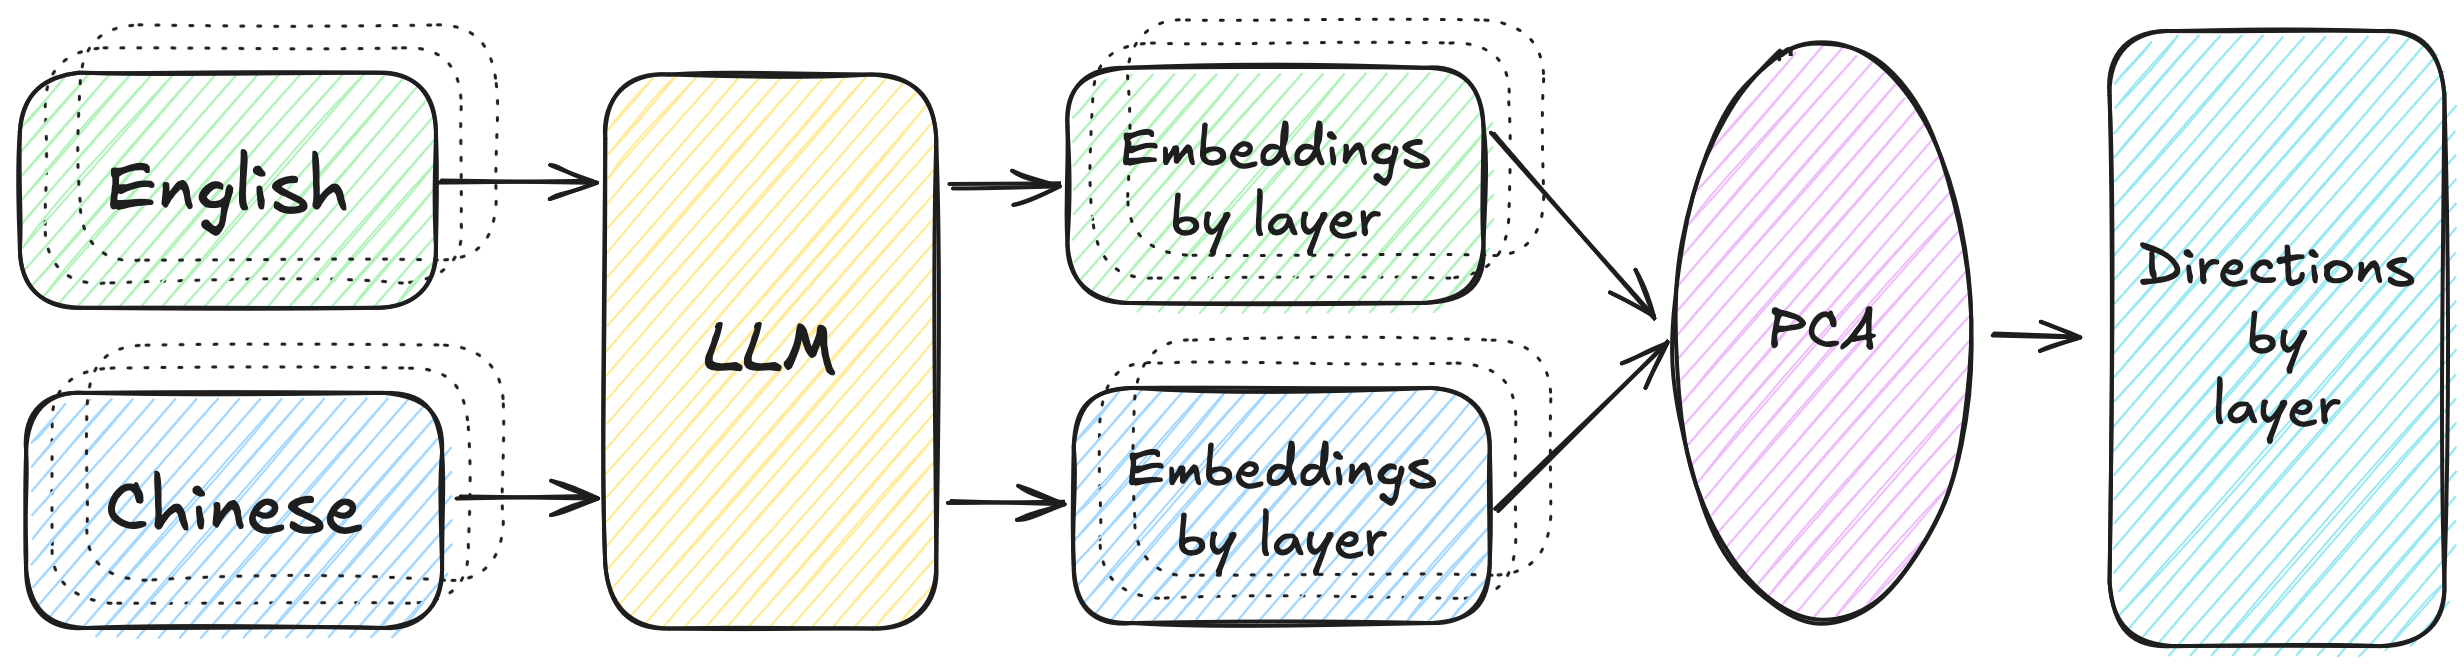
\includegraphics[width=1\linewidth]{images/language_steering_scheme.png}
  \caption{Language steering in hidden space: 1. Collect parallel translations of the same concepts; 2. LLM forward pass to get embeddings by layer; 3. Perform PCA by layer on the merged embeddings.}
  \label{fig:lang_steering_scheme}
\end{figure}

Our analysis shows language identity concentrates in final layers, with PC1 capturing most of the variance and enabling near-perfect language classification. We validate across Qwen2.5 and Llama-3.2 models on multiple language pairs (English, Spanish, Russian, Chinese, and Hindi), demonstrating reduced distributional divergence and substantially lower code-switching rates in generated text.

Code and data are released to facilitate further research \footnote{\url{https://github.com/fxlrnrpt/language-steering-in-latent-space}}.

\section{Results}
\label{sec:results}

\begin{figure*}[ht]
  \centering
  \begin{subfigure}[b]{0.48\linewidth}
    \centering
    
\includegraphics[width=1\linewidth]{images/language_map/multi/qwen/layer_28.pdf}
    \caption{Final layer language map (Qwen)}
    \label{fig:qwen_lang_map}
  \end{subfigure}
  \hfill
  \begin{subfigure}[b]{0.48\linewidth}
    \centering
    
\includegraphics[width=1\linewidth]{images/language_map/multi/llama/layer_16.pdf}
    \caption{Final layer language map (Llama)}
    \label{fig:llama_lang_map}
  \end{subfigure}
\end{figure*}

% \begin{figure*}[ht]
%   \centering
%   \begin{subfigure}[t]{0.24\linewidth}
%     \centering
%     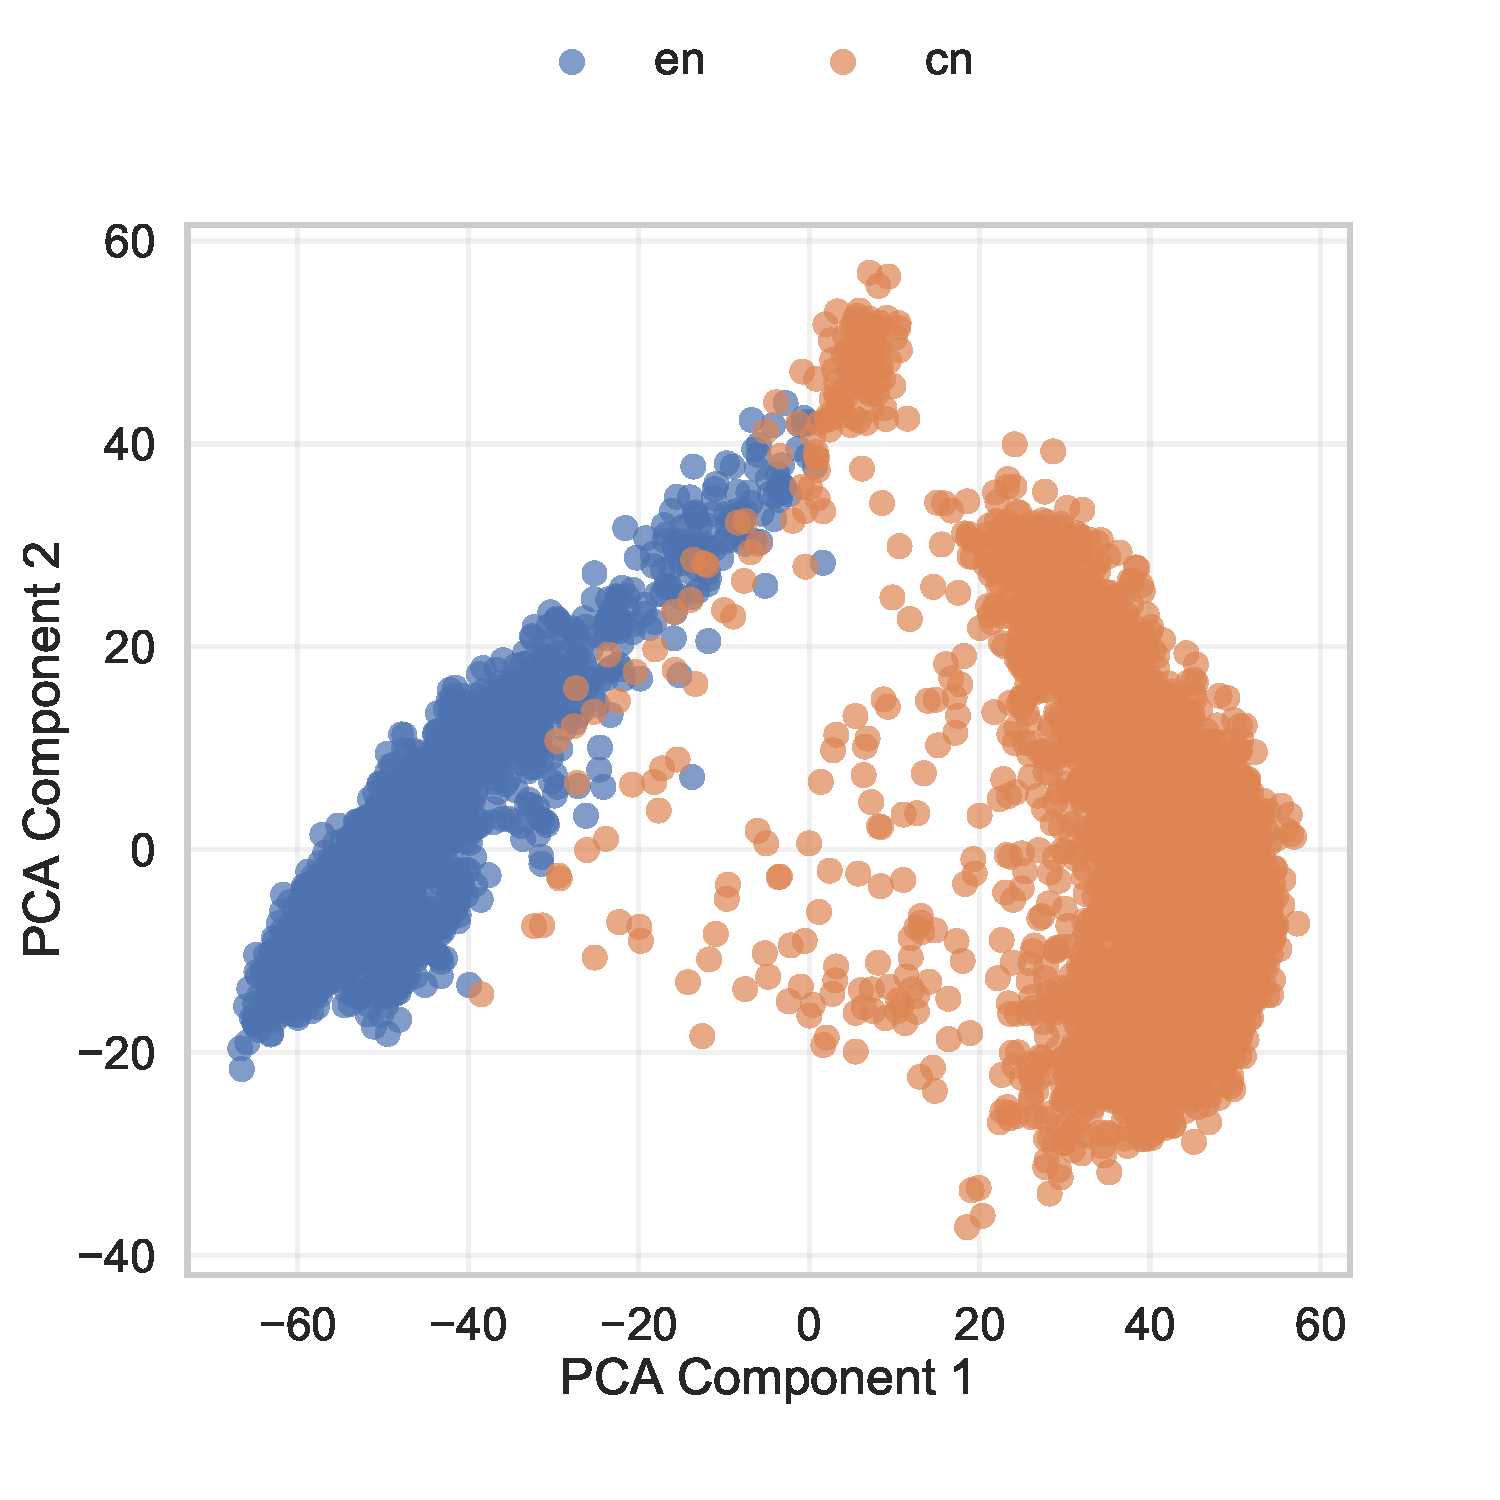
\includegraphics[width=1\linewidth]{images/language_map/en_cn/llama/layer_16.pdf}
%     \caption{English - Chinese}
%     \label{fig:llama_lang_map_en_cn}
%   \end{subfigure}
%   \hfill
%   \begin{subfigure}[t]{0.24\linewidth}
%     \centering
%     
\includegraphics[width=1\linewidth]{images/language_map/en_es/llama/layer_16.pdf}
%     \caption{English - Spanish}
%     \label{fig:llama_lang_map_en_es}
%   \end{subfigure}
%   \hfill
%   \begin{subfigure}[t]{0.24\linewidth}
%     \centering
%     
\includegraphics[width=1\linewidth]{images/language_map/en_ru/llama/layer_16.pdf}
%     \caption{English - Russian}
%     \label{fig:llama_lang_map_en_ru}
%   \end{subfigure}
%   \hfill
%   \begin{subfigure}[t]{0.24\linewidth}
%     \centering
%     
\includegraphics[width=1\linewidth]{images/language_map/en_hin/llama/layer_16.pdf}
%     \caption{English - Hindi}
%     \label{fig:llama_lang_map_en_hin}
%   \end{subfigure}
% \end{figure*}

We validate our approach on Qwen2.5-1.5B ~\cite{qwen2025qwen25technicalreport} and Llama-3.2-1B ~\cite{grattafiori2024llama3herdmodels}.

\subsection{Language direction identification}

We use Flores Plus \cite{nllb-24} dataset with 50 parallel samples for PCA fitting and 100 for validation. Figure~\ref{fig:qwen_lang_map} and~\ref{fig:llama_lang_map} show final-layer embeddings projected onto the first two PCs. Consistent with prior findings~\cite{conneau-etal-2020-emerging, wendler-etal-2024-llamas}, models organize identical content into tight, language-specific clusters with clear boundaries.

A simple logistic regression classifier trained only on the first principal component achieves near-perfect accuracy (0.96-1.00) across all language pairs and both models.

\subsection{Language steering}

We fit the steering module on Flores Plus with 200 parallel samples and test on 2,467 TED Talks samples with artificial code-switching.

Table~\ref{tab:kl} shows steering reduces KL divergence by 25-55\% across language pairs and models (38\% average for Qwen, 43\% for Llama).

\begin{table}[h]
  \centering
  \begin{tabular}{l l l}
    \hline
    Language pair & Qwen & Llama \\
    \hline
    English - Chinese & 10.15 $\rightarrow$ 4.52 & 9.05 $\rightarrow$ 4.77 \\
    English - Spanish & 7.25 $\rightarrow$ 4.90 & 6.52 $\rightarrow$ 3.48 \\
    English - Russian & 8.70 $\rightarrow$ 5.40 & 7.77 $\rightarrow$ 3.49 \\
    English - Hindi & 9.60 $\rightarrow$ 7.02 & 8.06 $\rightarrow$ 6.13 \\
    \hline
  \end{tabular}
  \caption{KL divergence (no steering $\rightarrow$ steering)}
  \label{tab:kl}
\end{table}

\subsection{Generation-based evaluation}
\label{sec:generation_eval}

To complement the distributional analysis above, we evaluate steering on actual text generation using Llama-3.2-1B. Across all four language pairs (English-Chinese/Spanish/Russian/Hindi), steering vectors lower the Code-Switching Index (CSI) from 0.59-0.81 (unsteered) to 0.01-0.23 while raising Target Language Consistency (TLC) to 0.77-0.99, with all differences significant at p < 0.001.

% \begin{table}[h]
%   \centering
%   \small
%   \begin{tabular}{l c c c c}
%     \hline
%     & \multicolumn{2}{c}{KL-optimized} & \multicolumn{2}{c}{CSI-optimized} \\
%     \cmidrule(lr){2-3} \cmidrule(lr){4-5}
%     Language pair & CSI ($\downarrow$) & TLC ($\uparrow$) & CSI ($\downarrow$) & TLC ($\uparrow$) \\
%     \hline
%     \multicolumn{5}{l}{\textit{Unsteered (code-switched input, no steering):}} \\
%     English - Chinese  & \multicolumn{2}{c}{0.64 / 0.36} & \multicolumn{2}{c}{---} \\
%     English - Spanish  & \multicolumn{2}{c}{0.62 / 0.38} & \multicolumn{2}{c}{---} \\
%     English - Russian  & \multicolumn{2}{c}{0.59 / 0.41} & \multicolumn{2}{c}{---} \\
%     English - Hindi    & \multicolumn{2}{c}{0.81 / 0.19} & \multicolumn{2}{c}{---} \\
%     \hline
%     \multicolumn{5}{l}{\textit{Steered:}} \\
%     English - Chinese  & 0.03 & 0.97 & 0.03 & 0.97 \\
%     English - Spanish  & 0.23 & 0.77 & 0.11 & 0.89 \\
%     English - Russian  & 0.02 & 0.98 & 0.01 & 0.99 \\
%     English - Hindi    & 0.04 & 0.96 & 0.01 & 0.99 \\
%     \hline
%   \end{tabular}
%   \caption{Generation-based code-switching metrics (Llama-3.2-1B, $n=500$). English-only baseline: CSI~$= 0.02$. All steered vs.\ unsteered differences significant at $p < 0.001$ (Wilcoxon signed-rank test).}
%   \label{tab:gen_results}
% \end{table}

% Bibliography entries for the entire Anthology, followed by custom entries
\bibliography{custom}
\bibliographystyle{plainnat}

%\clearpage

%\appendix
%\input{tex/appendix.tex}

\end{document}
